\documentclass[tikz,border=10pt]{standalone}
\usepackage{tkz-euclide} % 引入几何绘图增强包

\begin{document}
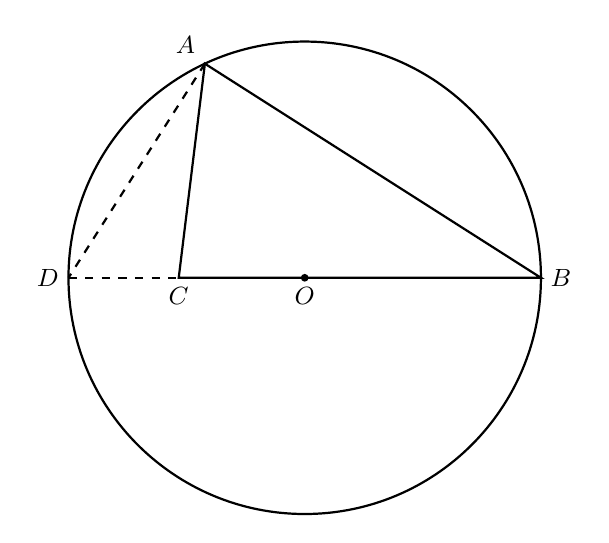
\begin{tikzpicture}[scale=2, font=\small]
    % 1. 定义基本参数（圆心和半径）
    \coordinate (O) at (0,0);
    \def\r{1.5} % 圆半径
    
    % 2. 定义圆周上的点
    \coordinate (D) at (-\r, 0);
    \coordinate (B) at (\r, 0);
    % A点通过极坐标定义，约在110度位置
    \coordinate (A) at (115:\r);
    
    % 3. 定义直径上的点 C (设定在 O 点左侧)
    \coordinate (C) at (-0.8, 0);

    % 4. 绘制圆形
    \draw[thick] (O) circle (\r);

    % 5. 绘制实绩线段 (三角形 ABC)
    \draw[thick] (A) -- (B) -- (C) -- cycle;
    % 绘制直径的右半部分（实线段 OB）
    \draw[thick] (C) -- (B);

    % 6. 绘制虚线辅助线 (AD 和 DC)
    \draw[dashed, thick] (A) -- (D);
    \draw[dashed, thick] (D) -- (C);

    % 7. 绘制关键点标记
    \fill (O) circle (0.7pt);
    
    % 8. 标注文字标签
    % 使用 anchor 自动调整位置避免覆盖线条
    \node[above left] at (A) {$A$};
    \node[right] at (B) {$B$};
    \node[below] at (C) {$C$};
    \node[left] at (D) {$D$};
    \node[below] at (O) {$O$};

\end{tikzpicture}
\end{document}